\documentclass[t]{beamer}


\usepackage[T1]{fontenc}
\usepackage[utf8]{inputenc}
%\usepackage[ngerman]{babel}
%\usepackage[babel,german=quotes]{csquotes}
\usepackage{graphicx}
\usepackage{color}
\usepackage{import}
% \usepackage{subfig}
%\usepackage[labelformat=empty]{caption}
\newcommand{\themepath}{../latex_templates/theme/}
\subimport{\themepath}{beamerthemefablab-4-3.sty}

\usepackage[font=large,labelfont=bf]{caption}

\begin{document}
% Title page


\date{\today}
\institute{FAU Fablab}
\title[Vorstellung]{Vorstellung des FAU Fablabs}
\author{} % TODO Namen der Vorstellenden eintragen
\frame[plain,c]{\titlepage} % plain-Option deaktiviert Kopf- und Fusszeile


% \captionsetup[subfloat]{labelformat=empty,font=large}

% \frame{\frametitle{Inhalt}\tableofcontents}

\begin{frame}
    \frametitle{Was ist das Fablab?}
    % Was, Wer, Wie, Wo
    \begin{itemize}
        \item Von Studenten betriebene offene Hightech-Werkstatt an der TechFak
        %\item Von Studenten für alle/jeden
        \item Umsetzung eigener Ideen bzw. Unterstützung von Forschung/Lehre
        \item Selber machen, lernen wie es geht -- keine Auftragsfertigung\\~
		\item Ziel: Bereitstellung von Technologien 
			\begin{itemize}
				\item Lasercutter
				\item 3D-Drucker
				\item Elektrowerkstatt mit Lötstationen, Platinenfertigung, Netzteilen, Messtechnik, ...
				\item Näh- und Stickmaschine
				\item CNC Fräse und CNC Drehbank\\~
			\end{itemize}
        \item Benutzung zum Selbstkostenpreis: nur Material und Verschleiß
		\item Angebot wird gut angenommen, vor Corona rund 40 Bezahlvorgänge pro Woche
        %\item Private Nutzung: selber zahlen
        %\item Für dieses Praktikum: auch Abrechnung mit dem Lehrstuhl möglich \\(Dazu erst beim Lehrstuhl nachfragen! Selber bezahlen, dann Kassenzettel beim Lehrstuhl einreichen.)
    \end{itemize}

\end{frame}

\begin{frame}{FAU Fablab}
    \begin{columns}
        \begin{column}[T]{0.25\textwidth}
            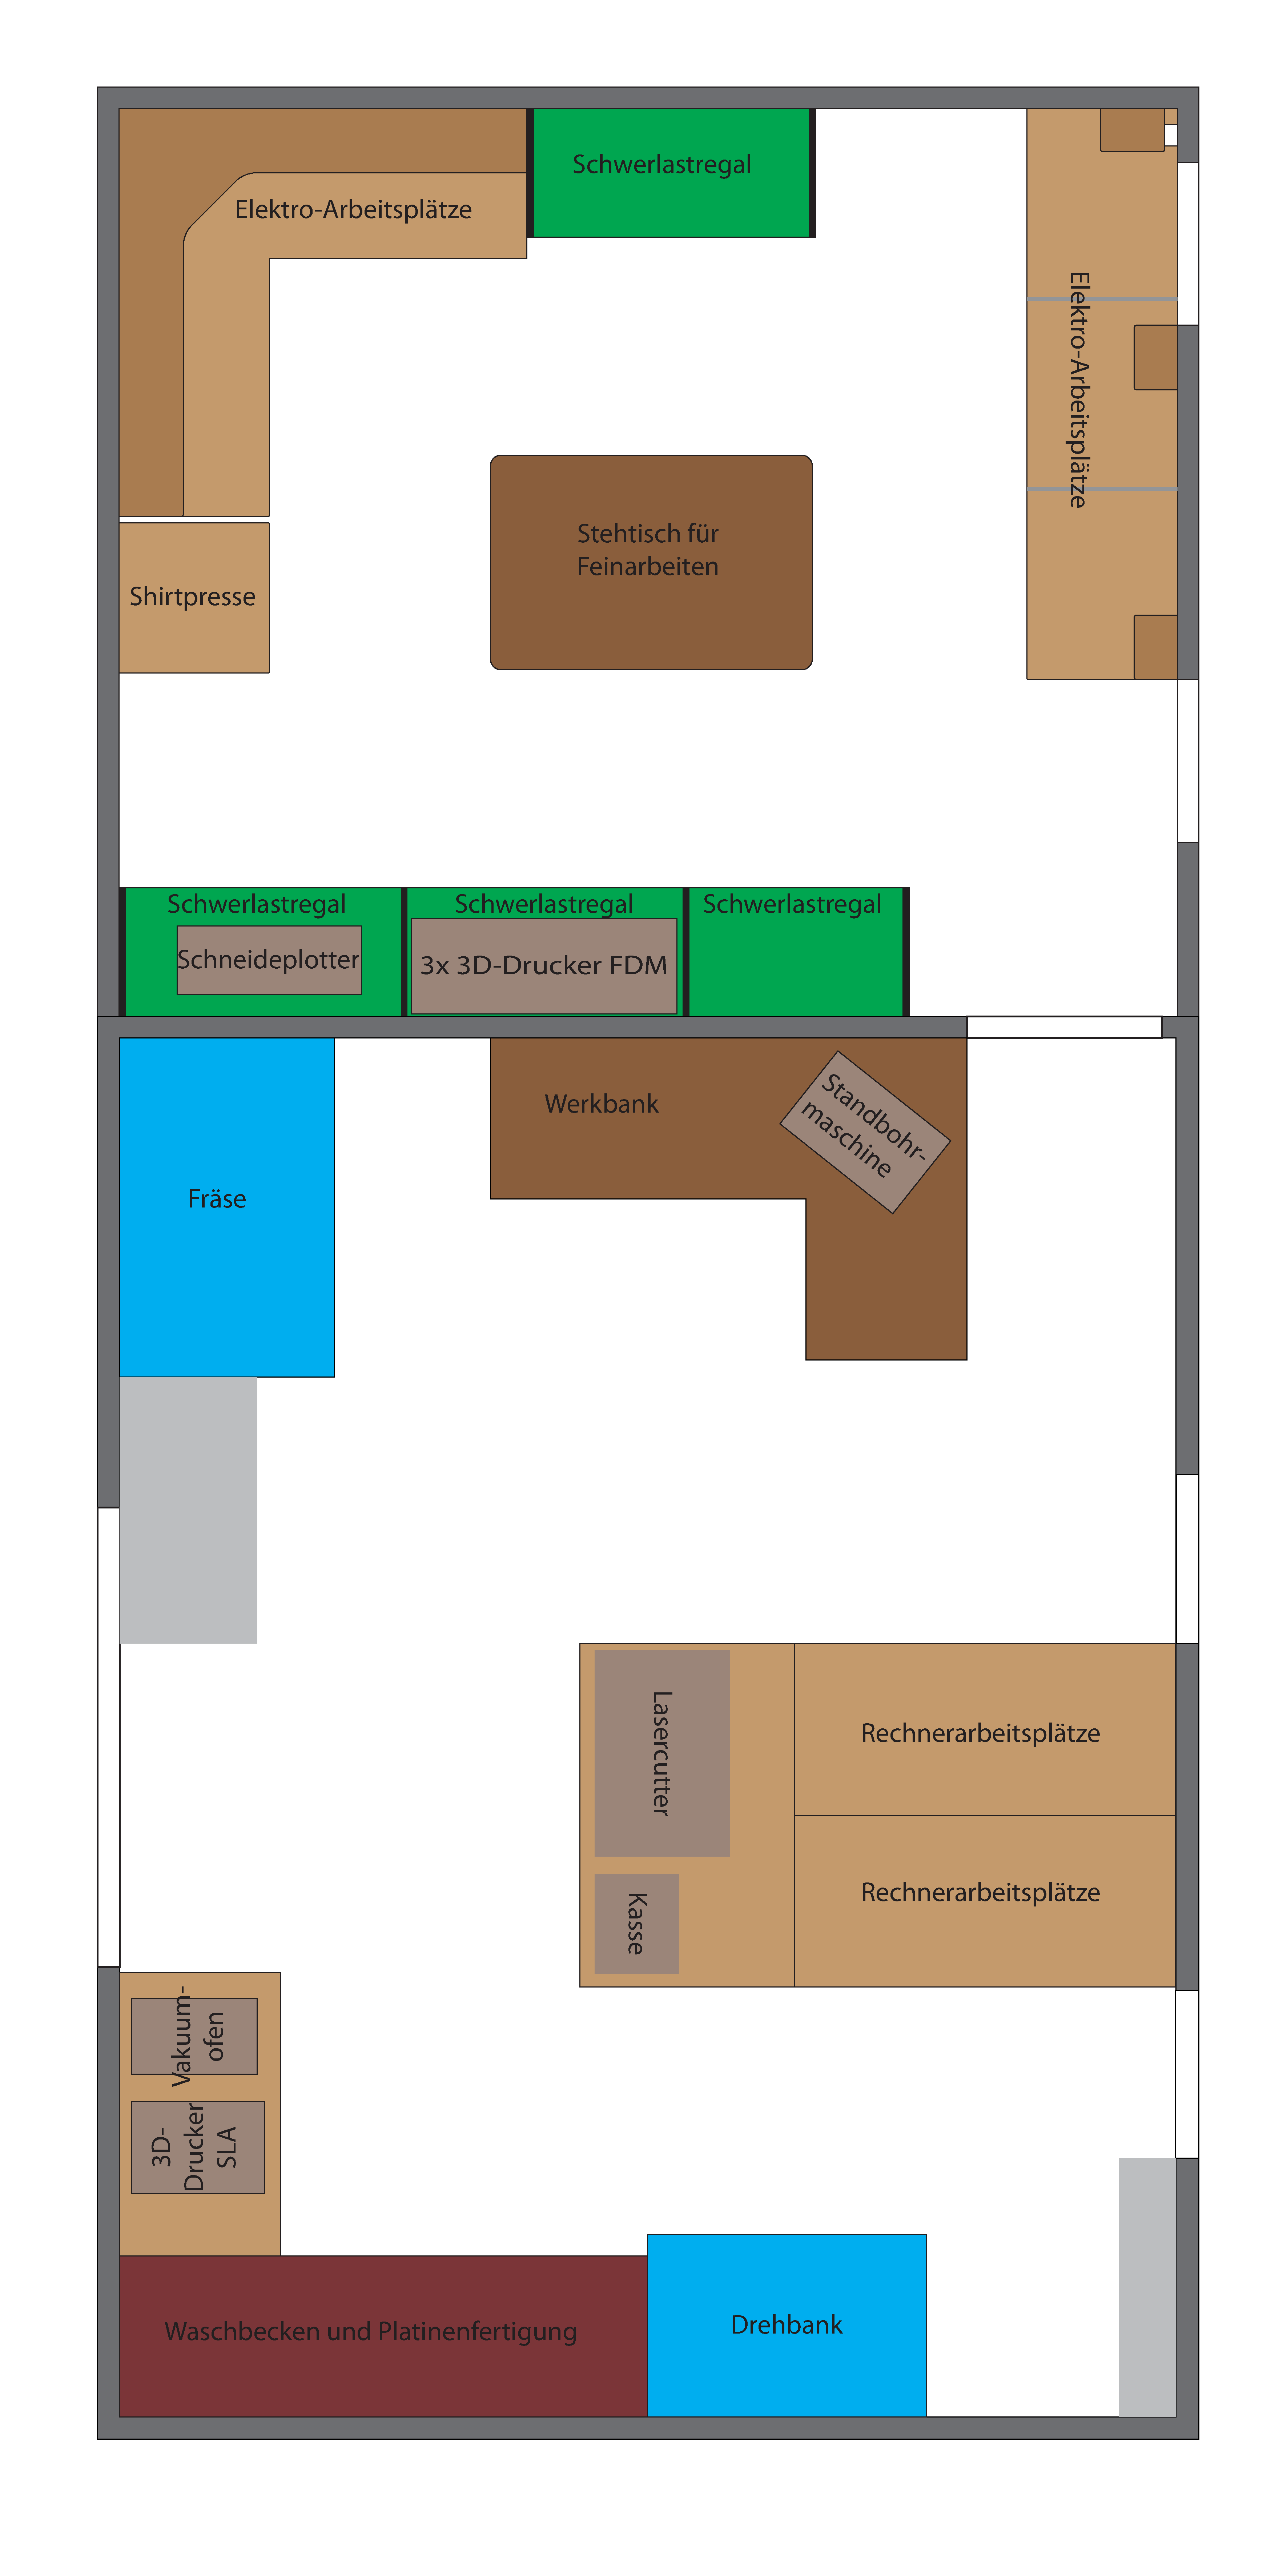
\includegraphics[height=0.9\textheight]{../img/fablabplan.pdf}
        \end{column}
        \begin{column}[T]{0.7\textwidth}
            \includegraphics[width=\textwidth,clip,trim=4cm 3cm 0cm 13cm]{../img/ewerkstatt.jpg}\\
            \includegraphics[width=\textwidth,clip,trim=0cm 5cm 0cm 7cm]{../img/hauptraum.jpg}
        \end{column}
    \end{columns}
\end{frame}

\begin{frame}{Antrag}
	\begin{itemize}
		\item Vier Gruppen\\~
		\item Ersatz für die bisher als Leihgabe bereitgestellte Stickmaschine
		\item Mechanikwerkstatt 
			\begin{itemize}
				\item Glasmessstäbe für den nicht-CNC Betrieb der Drehbank
				\item Monitorhalterungen 
			\end{itemize}
		\item Damphphasenlötanlage
		\item "Kleinere" Anschaffungen: 3D Scanner, Grafiktablet, ...\\~
		\item Antragssumme: 14.580,76 €
	\end{itemize}
\end{frame}

\end{document}
